% Comunicación entre los dispositivos cliente y el módulo central.
% Se compila por separado: pdflatex comunicacion_central.tex -> comunicacion_central.pdf
\documentclass[tikz,border=6pt]{standalone}
\usepackage[utf8]{inputenc}
\usepackage[T1]{fontenc}
\usepackage{cmbright}
\usetikzlibrary{arrows.meta,calc,fit,backgrounds}

\definecolor{azul}{RGB}{20,50,120}
\definecolor{flecha}{RGB}{25,80,190}
\definecolor{tarjeta}{RGB}{236,238,252}
\definecolor{borde}{RGB}{200,205,235}
\definecolor{cdatos}{RGB}{190,100,10}
\definecolor{capp}{RGB}{30,120,60}

\begin{document}
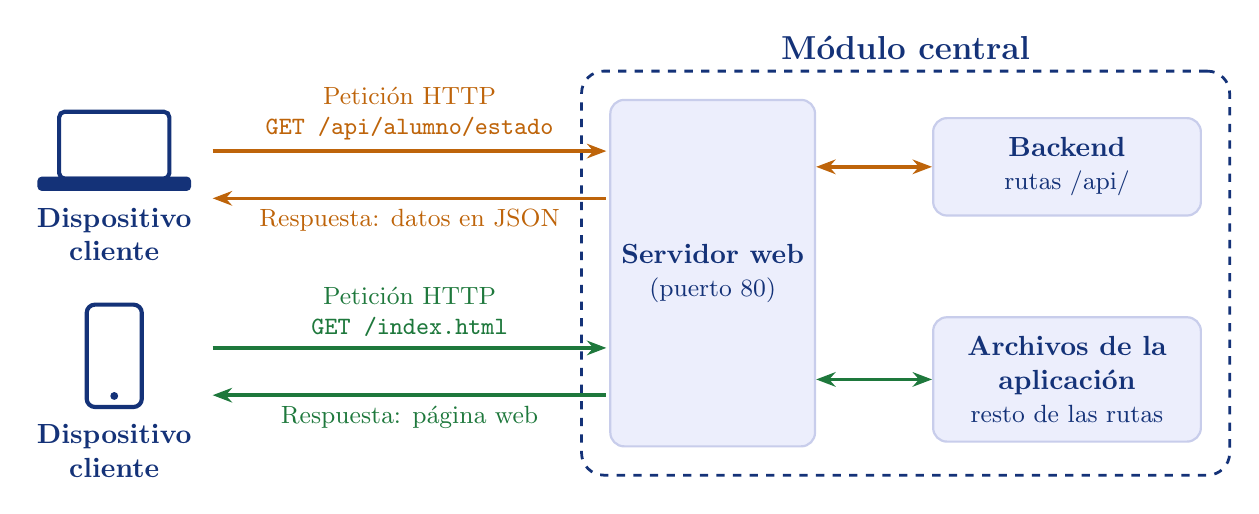
\begin{tikzpicture}[
    font=\normalsize,
    caja/.style={draw=borde, line width=0.8pt, fill=tarjeta, rounded corners=5pt,
                 inner sep=7pt, align=center, text=azul},
    msg/.style={font=\small, align=center},
    >={Stealth[length=7pt]}
]

% ---------------- Dispositivos cliente ----------------
% Computadora (camino de los datos)
\begin{scope}[shift={(0,1.45)}, azul, line width=1.5pt]
  \draw[rounded corners=2pt] (-0.7,-0.25) rectangle (0.7,0.6);
  \draw[rounded corners=1pt, fill=azul] (-0.95,-0.38) rectangle (0.95,-0.25);
\end{scope}
\node[text=azul, align=center, anchor=north] at (0,0.95) {\textbf{Dispositivo}\\\textbf{cliente}};

% Celular (camino de la aplicación)
\begin{scope}[shift={(0,-1.05)}, azul, line width=1.5pt]
  \draw[rounded corners=3pt] (-0.35,-0.65) rectangle (0.35,0.65);
  \fill (0,-0.51) circle (0.05);
\end{scope}
\node[text=azul, align=center, anchor=north] at (0,-1.8) {\textbf{Dispositivo}\\\textbf{cliente}};

% ---------------- Módulo central ----------------
\node[caja, minimum width=2.6cm, minimum height=4.4cm] (srv) at (7.6,0) {};
\node[text=azul, align=center] at (srv) {\textbf{Servidor web}\\{\small (puerto 80)}};

\node[caja, minimum width=3.4cm] (api) at (12.1,1.35) {\textbf{Backend}\\{\small rutas /api/}};
\node[caja, minimum width=3.4cm] (arch) at (12.1,-1.35) {\textbf{Archivos de la}\\\textbf{aplicación}\\{\small resto de las rutas}};

\begin{scope}[on background layer]
  \node[draw=azul, line width=1pt, dashed, rounded corners=8pt, inner sep=10pt,
        fit=(srv)(api)(arch)] (mc) {};
\end{scope}
\node[text=azul, font=\large\bfseries, anchor=south] at (mc.north) {Módulo central};

% ---------------- Camino de los datos ----------------
\draw[->, cdatos, line width=1.3pt] (1.25,1.55) -- node[msg, above] {Petición HTTP\\\texttt{GET /api/alumno/estado}} (6.25,1.55);
\draw[<-, cdatos, line width=1.3pt] (1.25,0.95) -- node[msg, below] {Respuesta: datos en JSON} (6.25,0.95);
\draw[<->, cdatos, line width=1.3pt] (srv.east |- api) -- (api.west);

% ---------------- Camino de la aplicación ----------------
\draw[->, capp, line width=1.3pt] (1.25,-0.95) -- node[msg, above] {Petición HTTP\\\texttt{GET /index.html}} (6.25,-0.95);
\draw[<-, capp, line width=1.3pt] (1.25,-1.55) -- node[msg, below] {Respuesta: página web} (6.25,-1.55);
\draw[<->, capp, line width=1.3pt] (srv.east |- arch) -- (arch.west);

\end{tikzpicture}
\end{document}
